% arara: xelatex
%% arara: xelatex


% https://koalatea.io/r-knn-regression/
% http://freerangestats.info/blog/2017/04/09/propensity-v-regression
% https://economics.stackexchange.com/questions/45335/what-is-the-difference-between-ate-and-att
% https://kosukeimai.github.io/MatchIt/articles/matching-methods.html


\documentclass[14pt,xcolor=dvipsnames]{beamer}


% !TEX root = om_metrics_14.tex

%\usepackage{epsdice} % dice 1-6 for probability :)

% \usepackage[absolute,overlay]{textpos}

% \usefonttheme[onlymath]{serif}

\usefonttheme{professionalfonts}
% by default beamer changes math fonts for better visibility for projection
% this professionalfonst theme removes this behavior


\usepackage[orientation=portrait,size=custom,width=25.4,height=19.05]{beamerposter}




%25,4 см 19,05 см размеры слайда в powerpoint

\usetheme{metropolis}
\metroset{
  %progressbar=none,
  numbering=none,
  subsectionpage=progressbar,
  block=fill
}

%\usecolortheme{seahorse}

\usepackage{xunicode} % хак для акцентов!
% https://tex.stackexchange.com/questions/28003/

\usepackage{fontspec}
\usepackage{polyglossia}
\setmainlanguage{russian}


% \usepackage{fontawesome5} % removed [fixed]
\setmainfont[Ligatures=TeX]{Myriad Pro}
% \setsansfont{Myriad Pro}




% why do we need \newfontfamily:
% http://tex.stackexchange.com/questions/91507/
\newfontfamily{\cyrillicfonttt}{Myriad Pro}
\newfontfamily{\cyrillicfont}{Myriad Pro}
%\newfontfamily{\cyrillicfontbs}{Myriad Pro}
\newfontfamily{\cyrillicfontsf}{Myriad Pro}


% https://tex.stackexchange.com/questions/175860/why-does-unicode-math-break-the-kerning-of-accents-in-combination-with-amssymb
% "You shouldn't be using amssymb together with unicode-math"
\usepackage{amsmath}
\usepackage{amsthm} % amssymb 


% https://tex.stackexchange.com/questions/483722/
% \usepackage[MnSymbol]{mathspec}  % Includes amsmath.
% \usepackage{mathspec}  % Includes amsmath.
% \setmathsfont(Digits,Latin,Greek,Symbols)[Numbers={Lining,Proportional}]{Latin Modern Math}
% mathspec must be loaded earlier than amsmath



%\usepackage{bm}

% \usepackage{fdsymbol} % \nperp

% \usepackage{unicode-math} % \symbf
% \setmathfont{Latin Modern Math}



\usepackage{centernot}

\usepackage{graphicx}

\usepackage{wrapfig}
% \usepackage{animate} % animations :)
% \usepackage{tikz}
%\usetikzlibrary{shapes.geometric,patterns,positioning,matrix,calc,arrows,shapes,fit,decorations,decorations.pathmorphing}
% \usepackage{pifont}
\usepackage{comment}
\usepackage[font=small,labelfont=bf]{caption}
\captionsetup[figure]{labelformat=empty}
% \includecomment{techno}



%Расположение

\setbeamersize{text margin left=15 mm,text margin right=5mm} 
\setlength{\leftmargini}{38 pt}

%\usepackage{showframe}
%\usepackage{enumitem}
% \setlist{leftmargin=5.5mm}


%Цвета от дирекции

\definecolor{dirblack}{RGB}{58, 58, 58}
\definecolor{dirwhite}{RGB}{245, 245, 245}
\definecolor{dirred}{RGB}{149, 55, 53}
\definecolor{dirblue}{RGB}{0, 90, 171}
\definecolor{dirorange}{RGB}{235, 143, 76}
\definecolor{dirlightblue}{RGB}{75, 172, 198}
\definecolor{dirgreen}{RGB}{155, 187, 89}
\definecolor{dircomment}{RGB}{128, 100, 162}

\setbeamercolor{title separator}{bg=dirlightblue!50, fg=dirblue}

%Цвета блоков

% Голубой блок!
\setbeamercolor{block title}{bg=dirblue!30,fg=dirblack}
\setbeamercolor{block title example}{bg=dirlightblue!50,fg=dirblack}
\setbeamercolor{block body example}{bg=dirlightblue!20,fg=dirblack}

\AtBeginEnvironment{exampleblock}{\setbeamercolor{itemize item}{fg=dirblack}}
%\setbeamertemplate{blocks}[rounded][shadow]

% Набор команд для удобства верстки

% Набор команд для структуризации

%\newcommand{\quest}{\faQuestionCircleO}
%\faPencilSquareO \faPuzzlePiece \faQuestionCircleO  \faIcon*[regular]{file} {\textcolor{dirblue}
%\newcommand{\quest}{\textcolor{dirblue}{\boxed{\textbf{?}}}
%\newcommand{\task}{\faIcon{tasks}}
%\newcommand{\exmpl}{\faPuzzlePiece}
%\newcommand{\dfn}{\faIcon{pen-square}}
%\newcommand{\quest}{\textcolor{dirblue}{\faQuestionCircle[regular]}}
%\newcommand{\acc}[1]{\textcolor{dirred}{#1}}
%\newcommand{\accm}[1]{\textcolor{dirred}{#1}}
%\newcommand{\acct}[1]{\textcolor{dirblue}{#1}}
%\newcommand{\acctm}[1]{\textcolor{dirblue}{#1}}
%\newcommand{\accex}[1]{\textcolor{dirblack}{\bf #1}}
%\newcommand{\accexm}[1]{\textcolor{dirblack}{ \mathbf{#1}}}
%\newcommand{\acclp}[1]{\textcolor{dirorange}{\it #1}}
\newcommand{\todo}[1]{\textcolor{dircomment}{\bf #1}}
%\newcommand{\graylink}[1]{{\fontsize{11}{12}\selectfont \textcolor{gray}{#1}}}
%\newcommand{\figcaption}[1]{{\fontsize{18}{20}\selectfont #1}}


\newcommand{\videotitle}[1]{
    {\fontsize{33}{30}\selectfont \textcolor{dirblue}{\textbf{#1}} }

    %\todo{название видеофрагмента}
}

\newcommand{\lecturetitle}[1]{
  {\fontsize{33}{30}\selectfont \textcolor{dirblue}{\textbf{#1}} }

    %\todo{название лекции}
}





%\newcommand{\spcbig}{\vspace{-10 pt}}
%\newcommand{\spcsmall}{\vspace{-5 pt}}

%\usepackage{listings}
%\lstset{
%xleftmargin=0 pt,
%  basicstyle=\small, 
%  language=Python,
  %tabsize = 2,
%  backgroundcolor=\color{mc!20!white}
%}



%\newcommand{\mypart}[1]{\begin{frame}[standout]{\huge #1}\end{frame}}

\setbeamercolor{background canvas}{bg=}

% frame title setup
\setbeamercolor{frametitle}{bg=,fg=dirblue}
\setbeamertemplate{frametitle}[default][left]

\addtobeamertemplate{frametitle}{\hspace*{0.1 cm}}{\vspace*{0.25cm}}


%Шрифты
\setbeamerfont{frametitle}{family=\rmfamily,series=\bfseries,size={\fontsize{33}{30}}}
\setbeamerfont{framesubtitle}{family=\rmfamily,series=\bfseries,size={\fontsize{26}{20}}}


% удобнее знать номер слайда, чтобы вносить правки!  

\setbeamercolor{footline}{fg=dircomment}
\setbeamerfont{footline}{series=\bfseries, size={\fontsize{12}{14}}}
%\setbeamertemplate{footline}[page number]


\defbeamertemplate{footline}{custom footline}
{%
  \hspace*{\fill}%
  \usebeamercolor[fg]{page number in head/foot}%
  \usebeamerfont{page number in head/foot}%
  page: \insertpagenumber\,/\,\insertpresentationendpage%
  \hspace{20pt}%
  slide: \insertframenumber\,/\,\inserttotalframenumber%
  %\hspace*{\fill}
  \vskip2pt%
}
%\setbeamertemplate{footline}[custom footline]

\usepackage{physics}
\usepackage[makeroom]{cancel}



% tikz block

\usepackage{pgfplots}
\pgfplotsset{compat=newest}

\usepackage{tikz}
\usetikzlibrary{calc}
\usetikzlibrary{quotes,angles}
\usetikzlibrary{arrows}
\usetikzlibrary{arrows.meta}
\usetikzlibrary{positioning,intersections,decorations.markings}
\usetikzlibrary{patterns}

\usepackage{tkz-euclide} 
%\tikzset{>=latex}

\tikzset{cross/.style={cross out, draw=black, minimum size=2*(#1-\pgflinewidth), inner sep=0pt, outer sep=0pt},
%default radius will be 1pt. 
cross/.default={5pt}}

\colorlet{veca}{red}
\colorlet{vecb}{blue}
\colorlet{vecc}{olive}


\newcommand{\grid}{\draw[color=gray,step=1.0,dotted] (-2.1,-2.1) grid (9.6,6.1)}

% end tikz block

\newcommand{\R}{\mathbb{R}}
\newcommand{\Rot}{\mathrm{R}}
\newcommand{\HH}{\mathrm{H}}
\newcommand{\Id}{\mathrm{I}}
\newcommand{\RR}{\mathbb{R}}
\newcommand{\ZZ}{\mathbb{Z}}
\newcommand{\la}{\lambda}
\let\P\relax
\newcommand{\P}{\mathbb{P}}
\newcommand{\E}{\mathbb{E}}

\newcommand{\cN}{\mathcal{N}}
\newcommand{\dN}{\mathcal{N}}

\newcommand{\qL}{q_{\text{left}}}
\newcommand{\qR}{q_{\text{right}}}



\newcommand{\ba}{\mathbf{a}}
\newcommand{\be}{\mathbf{e}}
\newcommand{\bb}{\mathbf{b}}
\newcommand{\bc}{\mathbf{c}}
\newcommand{\bd}{\mathbf{d}}
\newcommand{\bx}{\mathbf{x}}
\newcommand{\bff}{\mathbf{f}} % \bf is already def
\newcommand{\bv}{\mathbf{v}}
\newcommand{\bzero}{\mathbf{0}}



\DeclareMathOperator{\Var}{Var}
\DeclareMathOperator{\sVar}{sVar}
\DeclareMathOperator{\Cov}{Cov}
\DeclareMathOperator{\sCov}{sCov}
\DeclareMathOperator{\sCorr}{sCorr}
\DeclareMathOperator{\pCorr}{pCorr}
\DeclareMathOperator{\Corr}{Corr}
\DeclareMathOperator{\Med}{Med}
\let\L\relax
\DeclareMathOperator{\L}{L}


\DeclareMathOperator{\plim}{plim}
\DeclareMathOperator{\sign}{sign}


\newcommand{\graylink}[1]{{\fontsize{11}{12}\selectfont \textcolor{gray}{#1}}}
\newcommand{\figcaption}[1]{{\fontsize{18}{20}\selectfont #1}}





\begin{document}


\begin{frame} % название лекции


\lecturetitle{Вопросы и ответы}

\end{frame}


% !TEX root = ../om_ts_09.tex

\begin{frame} % название фрагмента

\videotitle{Много сезонных составляющих}

\end{frame}



\begin{frame}{Много сезонных составляющих: план}
  \begin{itemize}[<+->]
    \item Наложение \alert{нескольких частот}.
    \item Краткое напоминание STL.
    \item MSTL = STL \alert{много раз}.
  \end{itemize}

\end{frame}

\begin{frame}
  \frametitle{Число звонков в банк}

  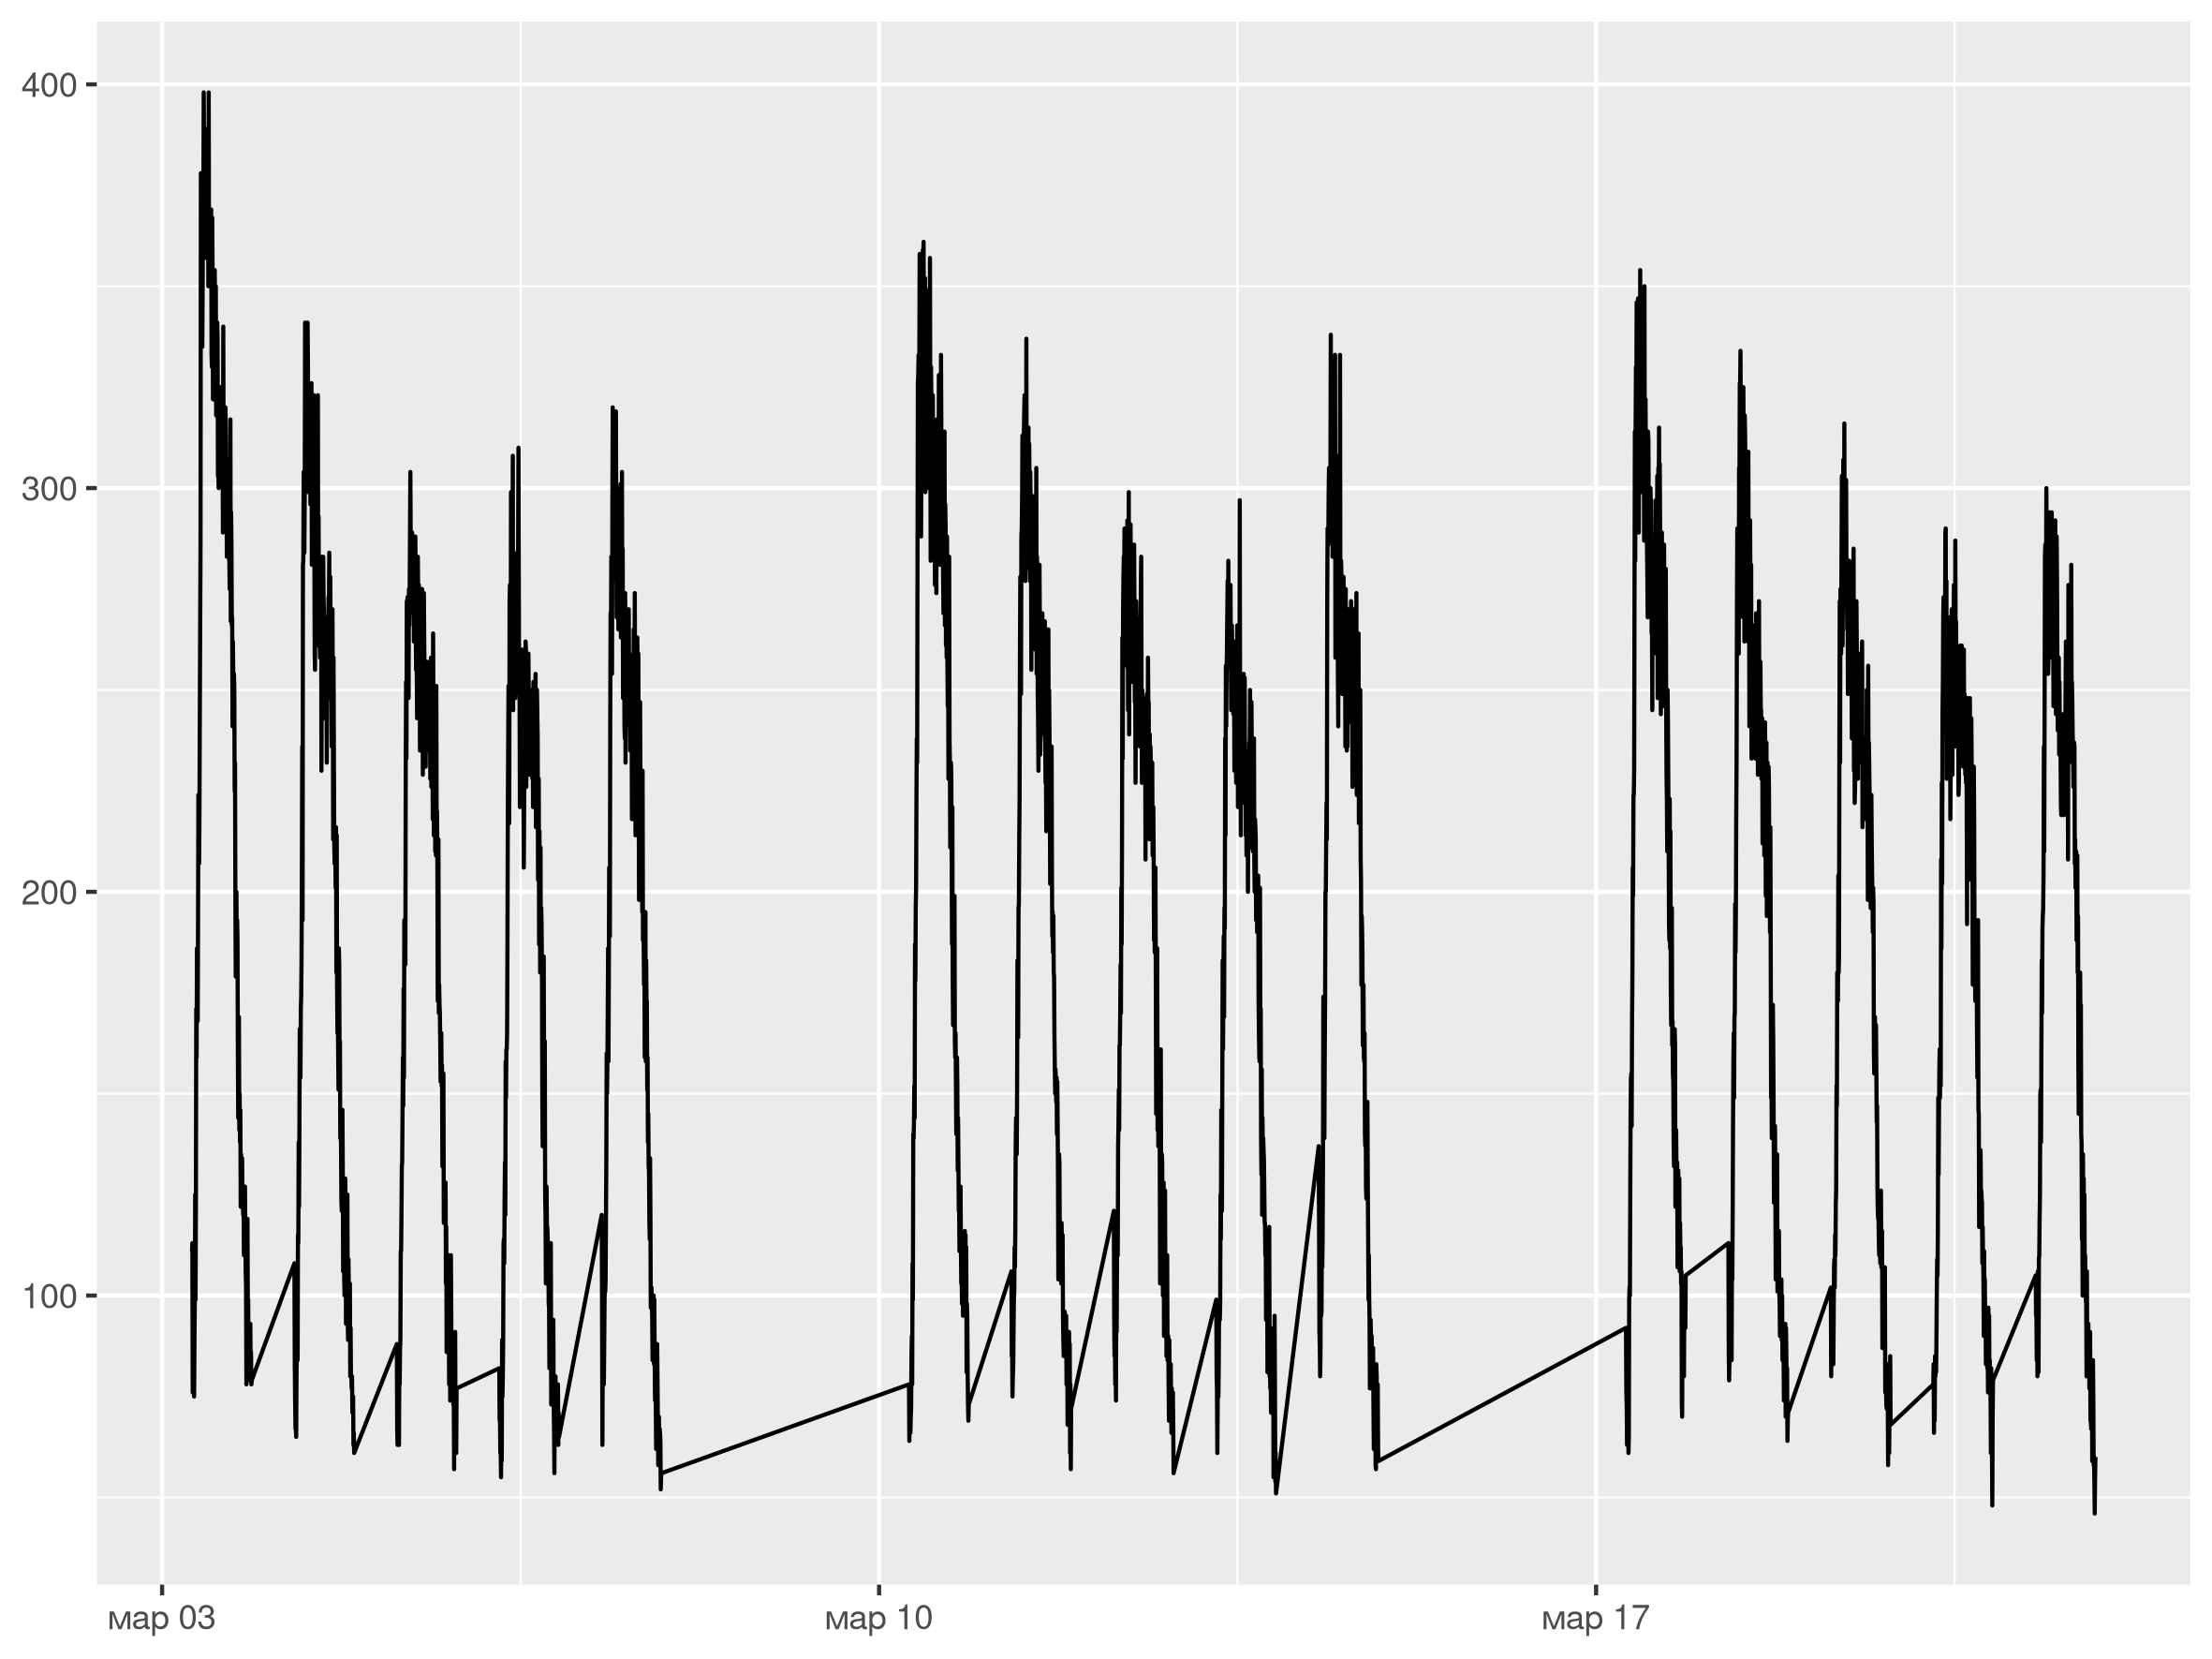
\includegraphics[width=\textwidth]{pictures/om_ts_09-006.png}

  
\end{frame}

\begin{frame}
  \frametitle{Что делать со сложной сезонностью?}

  \begin{itemize}[<+->]
    \item Использовать \alert{подходящую} модель:
    
    ARIMA + предикторы Фурье, PROPHET, TBATS, \ldots

    \item Разложить ряд на \alert{много} составляющих:
    
    \[
      y_t = trend_t + seas_t^{(1)} + seas_t^{(2)} + remainder_t
    \]
  \end{itemize}
  

\end{frame}


\begin{frame}{Вспоминаем STL}

  \alert{На входе:}
  
  Ряд $y_t$.
  \pause
  \begin{itemize}
    \item $n_p$ — периодичность сезонности, например, $n_p=12$. \pause 
    \item $n_l$ — сила сглаживания низкочастотного фильтра.   \pause
    \item $n_s$ — сила сглаживания сезонных подряд\textit{о}в. \pause
    \item $n_t$ — сила сглаживания при выделении тренда.     
  \end{itemize}

  \pause
  \alert{На выходе:}
  
  Разложение $y_t = trend_t + seas_t + remainder_t$.  
\end{frame}
  
\begin{frame}
  \frametitle{Применим STL последовательно!}

  \begin{enumerate}[<+->]
    \item \alert{Первичное} выделение сезонных компонент. 
    \item \alert{Корректировка} сезонных компонент. 
    \item Добываем тренд и остаток. 
  \end{enumerate}

\end{frame}



\begin{frame}
  \frametitle{MSTL = STL много раз!}

  Шаг 1. Первичное выделение сезонных компонент. 

  \begin{enumerate}[<+->]
    \item Запустим STL для выделения сезонности \alert{высокой частоты}. 
    
    Запомним выделенную компоненту $seas_t^{(1)}$ и удалим её из ряда, $y_t^{(-1)} = y_t - seas_t^{(1)}$. 

    \item Запустим STL для выделения сезонности \alert{средней частоты}. 
    
    Запомним выделенную компоненту $seas_t^{(2)}$ и удалим её из ряда, $y_t^{(-1,2)}= y_t^{(-1)} - seas_t^{(2)}$. 

    \item \ldots

  \end{enumerate}

\end{frame}



\begin{frame}
  \frametitle{Уточняем сезонные компоненты}

  Шаг 2. Корректировка сезонных компонент. 

  \begin{enumerate}[<+->]
    \item Временно \alert{возвращаем} в полностью очищенный ряд найденную \alert{сезонность} высокой частоты.
    
    Запускаем STL и получаем \alert{уточнённую компоненту} $seas_t^{(1)}$, удаляем её из ряда и получаем \alert{уточнённый очищенный ряд}. 

    \item Временно \alert{возвращаем} в полностью очищенный ряд найденную \alert{сезонность} средней частоты.
    
    Запускаем STL и получаем \alert{уточнённую компоненту} $seas_t^{(2)}$, удаляем её из ряда и получаем \alert{уточнённый очищенный ряд}. 

    \item \ldots

  \end{enumerate}

\end{frame}



\begin{frame}
  \frametitle{Завершаем алгоритм}

  Шаг 3. Добываем тренд и остаток. 

  \alert{Тренд} и \alert{остаток} берем из самого \alert{последнего} STL разложения, уточнявшего сезонные компоненты. 
  
\end{frame}


\begin{frame}{Много сезонных составляющих: итоги}

  \begin{itemize}[<+->]
    \item \alert{MSTL} — быстрый и устойчивый алгоритм разложения ряда.
    \item Теоретически \alert{MSTL} может работать с пропусками.
    \item Есть другие алгоритмы: ARIMA + предикторы Фурье, TBATS, PROPHET, \ldots
  \end{itemize}
\end{frame}


% !TEX root = ../om_ts_09.tex

\begin{frame} % название фрагмента

\videotitle{Данные прерывающиеся нулями}

\end{frame}



\begin{frame}{Данные прерывающиеся нулями: план}
  \begin{itemize}[<+->]
    \item Нули в данных.
    \item Алгоритм Кростона. 
  \end{itemize}

\end{frame}

\begin{frame}
  \frametitle{Откуда нули в данных?}

  Счётные данные с \alert{небольшим} ожиданием: 
  \begin{itemize}[<+->]
    \item Ежедневное количество пожаров в небольшое городе.
    \item Еженедельное количество написанных писателем романов. 
    \item \ldots
  \end{itemize}
  
\end{frame}

\begin{frame}
  \frametitle{Как моделировать?}

  \begin{itemize}[<+->]
    \item Специальные модели для счётных данных. 
    
    Используют распределение \alert{Пуассона}, \alert{отрицательное биномиальное}, \ldots

    \item Простой алгоритм Кростона. 
    
    Подходит для \alert{несезонных} данных, основан на \alert{экспоненциальном сглаживании}. 
  \end{itemize}

  

\end{frame}


\begin{frame}
  \frametitle{Напоминание про ETS(ANN)}

  Уравнения модели:
  \[
  \begin{cases}
  y_t = \ell_{t-1} + u_t  \\
  \ell_t = \ell_{t-1} + \alpha u_t \\
  \end{cases}
  \]
  \pause
  \[
  \ell_t = \alpha y_t + (1 - \alpha) \ell_{t-1}
  \]
  \pause 
  Прогноз на 1 шаг вперёд:
  \[
  \hat y_{t+1} = \alpha y_t + (1-\alpha )\hat y_{t}.
  \]
\end{frame}


\begin{frame}{Алгоритм Кростона}
  
  Шаг 1. Разобъём исходный ряд $(y_t)$
  \[
   3, 0, 2, 0, 0, 4, 0, 0, 0, 3, 0, 1, \ldots
  \] \pause
  на ряд \alert{положительных} значений $(q_t)$
  \[
  3, 2, 4, 3, 1, \ldots  
  \]
  и \alert{длины нулевых промежутков} $(a_t)$:
  \[
  1, 2, 3, 1, \ldots   
  \]
  \pause 

  Шаг 2. Применим простое экспоненциальное сглаживание.
  \[
\begin{cases}
  \hat q_{t+1} = \alpha_q q_t + (1-\alpha_q )\hat q_{t} \\
  \hat a_{t+1} = \alpha_a a_t + (1-\alpha_a )\hat a_{t}
\end{cases}
  \]
  \pause 
  Параметры: $\alpha_a$, $\alpha_q$, $\hat a_{0}$, $\hat q_{0}$.


\end{frame}
  

\begin{frame}
  \frametitle{Прогнозирование}

  Из алгоритма Кростона можно извлечь:
  \begin{itemize}[<+->]
    \item $\hat q_{T+1}$ — прогноз следующего ненулевого числа. 
    \item $\hat a_{T+1}$ — прогноз длины нулевого промежутка. 
    \item $\hat y_{T+1} = \hat q_{T+1} / \hat a_{T+1}$ — прогноз для исходного ряда. 
  \end{itemize}
  
\end{frame}

\begin{frame}
  \frametitle{Сравнение прогнозов}

  Используйте \alert{MASE}:
    \[
      MASE  = \frac{\abs {q_{T+1}} + \abs{q_{T+2}}+ \ldots + \abs{q_{T+H}} }{H},
  \]  
  где 
  \begin{itemize}
    \item $e_t$ — ошибка прогноза;
    \item $q_t = \frac{e_t}{MAE^{naive}}$ — ошибка прогноза,
    отмашстабированная на среднюю абсолютную ошибку наивного прогноза. 
  \end{itemize}
\end{frame}


\begin{frame}{Данные прерывающиеся нулями: итоги}

  \begin{itemize}[<+->]
    \item Как правило, много нулей в \alert{счётных} данных.
    \item Алгоритм Кростона подойдёт для \alert{несезонных} данных. 
    \item Алгоритм Кростона \alert{нестатический}: нет прогнозных интервалов. 
  \end{itemize}
\end{frame}


% !TEX root = ../om_ts_09.tex

\begin{frame} % название фрагмента

\videotitle{Сравнение прогнозов}

\end{frame}



\begin{frame}{Сравнение прогнозов: план}
  \begin{itemize}[<+->]
    \item Тест Диболда-Мариано.
    \item RC-тест Уайта.
    \item SPA-тест Хансена. 
  \end{itemize}

\end{frame}

\begin{frame}
  \frametitle{Тест Диболда-Мариано}

  \begin{itemize}[<+->]
    \item Предназначен для сравнения \alert{двух} прогнозов.
    \item Сравнивает прогнозы на \alert{заданный горизонт} прогнозирования $h$.
    \item Не является оптимальным для \alert{сравнения моделей}. 
    \item Не подходит для \alert{попарного} сравнения множества прогнозов.
  \end{itemize}
  
\end{frame}

\begin{frame}
  \frametitle{Предпосылки DM-теста}

  Рассмотрим \alert{разницу потерь} двух прогнозов:
  \[
  d_t = e_{A,t}^2 - e_{B,t}^2, \quad e_{\text{Model},t} = \hat y_{\text{Model},t} - y_t;
  \]
  \pause
  Разница $d_t$ предполагается \alert{стационарной}:\pause
  \[
  \E(d_t) = \mu_d,
  \]
  \pause 
  \[
  \Cov(d_t, d_{t-k}) = \gamma_k,    
  \] \pause
  В частности,
  \[
  \Var(d_t) = \gamma_0.    
  \]
  
\end{frame}

\begin{frame}
    \frametitle{Способ тестирования}
    При верной $H_0: \mu_d = 0$:
    \[
       DM = \frac{\bar d}{se(\bar d)} \to \cN(0;1),
    \]
    где $se^2(\bar d)$ — состоятельная оценка для $\Var(\bar d)$.
    \pause 
    На практике оценивают регрессию на константу
    \[
    \hat d_t = \hat \beta_1
    \]
    \pause 
    Получают $\hat\beta_1 = \bar d$ и используют \alert{робастные стандартные ошибки},
    \[
        DM = \frac{\hat \beta_1}{se_{HAC}(\hat\beta_1)}.
    \]

\end{frame}


\begin{frame}
    \frametitle{RC-тест Уайта}

    RC = Reality Check, проверка реальностью. 
    \pause 

    \begin{itemize}
        \item Предназначен для сравнения \alert{множества} прогнозов с эталонным. \pause
        \item Сравнивает прогнозы на \alert{заданный горизонт} прогнозирования $h$. \pause
        \item Не является оптимальным для \alert{сравнения моделей}. \pause
      \end{itemize}

      $H_0$: ни один из прогнозов не обыгрывает эталонный прогноз. 

      $H_a$: хотя бы один из прогнозов лучше. 
\end{frame}

\begin{frame}
    \frametitle{Обозначения}
    
    \begin{itemize}
        \item $e_{jt} = \hat y_{jt} - y_t$ — ошибки прогноза модели $j$; \pause
        \item $d_{jt} = e_{jt}^2 - e_{\text{bench}, t}^2$ — разница потерь по сравнению с эталонным прогнозом. \pause
        \item $\bar d_j$ — средняя разница потерь модели $j$. \pause
        \item Статистика теста $RC = \max_j \bar d_j$.  
    \end{itemize}    
    \pause 
    Гипотезы:
    $H_0$: $\max_j \E(d_jt) \leq 0$. 

    $H_a$: $\max_j \E(d_jt) > 0$.
\end{frame}

\begin{frame}
    \frametitle{Запускаем бутстрэп}

    \begin{enumerate}
        \item По 
    \end{enumerate}
    

\end{frame}


\begin{frame}
    \frametitle{Вариации}

    Есть \alert{много} вариаций этого подхода. 


    

\end{frame}



\begin{frame}
    \frametitle{Почему сравнение прогнозов?}

    \alert{Тонкий нюанс}: сравнение прогнозов и сравнение моделей — разные задачи. 
    \pause
    Модель может сильно выигрывать \alert{по простоте} и немного проигрывать по прогнозам.
    \pause 
    На малой выборке \alert{потеря информации} о качестве прогнозов на обучающей выборке существенна. 
\end{frame}


\begin{frame}{Сравнение прогнозов: итоги}

  \begin{itemize}[<+->]
    \item Тест Диболда-Мариано подходит для сравнения \alert{двух} прогнозов. 
    \item SPA-тест и RC-тест подходят для сравнения \alert{множества} прогнозов. 
    \item Лучше использовать \alert{SPA-тест} Хансена. 
    \item Иногда названия \alert{SPA} и \alert{RC} путают. 
    \item SPA-тест используют, например, для сравнения \alert{торговых стратегий}. 
  \end{itemize}
\end{frame}



\end{document}
